\subsection{Verwandte Forschung}
\label{sec:VerwandteForschung}

Um räumlich-zeitliche Zusammenhänge in Datensätzen durch ein \acrshort{nn} zu erlernen existieren verschiedene Architekturen.
Im von Jiang et al. verfassten Paper \cite{DLTraff} befindet sich ein detaillierter Vergleich vieler dieser Architekturen anhand ihrer Ansätze und Performance.
Zwei weit verbreitete Beispiele werden im folgenden zusammengefasst.

\textbf{ST-ResNet} wird in \cite{STResNetOriginal} definiert und ist eines der populärsten Modelle für räumlich-zeitliche Vorhersagen.
Jiang et al. machen dies an der Anzahl der Paper fest, die Referenzen auf \cite{STResNetOriginal} enthalten.
Der Anwendungsfall für den ST-ResNet konzipiert wurde, ist die Vorhersage der Bewegung von Menschenmassen (engl. \emph{crowd flow}).
Dabei ist es egal, wie sich die Menschen bewegen.
So kann ST-ResNet beispielsweise nicht nur auf Fußgänger angewendet werden, sondern auch auf Leihfahrräder, Taxis oder Verkehr allgemein.
Ein Datensatz, für den ST-ResNet ursprünglich konzipiert wurde, besteht aus einem Raster über viele Zeitschritte.
Pro Zeitschritt sind jeder Zelle zwei Werte zugeordnet: die Anzahl an Menschen, die die Zelle betreten (engl. \emph{inflow}) und die Anzahl an Menschen, die die Zelle verlassen (engl. \emph{outflow}).
Dies ist ein Beispiel für einen Datensatz mit zwei Kanälen.
Für die Architektur von ST-ResNet haben sich Zhang et al. genau überlegt, welche räumlichen und zeitlichen Zusammenhänge in den Daten vorhanden sein könnten.
Sie stellen zunächst fest, dass der Inflow einer Zelle abhängig ist vom Outflow der benachbarten Zellen.
Es können jedoch auch Zusammenhänge zu weiter entfernten Zellen bestehen, da es in größeren Städten normalerweise ein U-Bahn Netz gibt, welches weiter entfernte Zellen direkt miteinander verbindet.
Bei den zeitlichen Zusammenhängen handelt es sich um verschieden große Zeitspannen.
Zhang et al. führen je Beispiele für Zusammenhänge innerhalb eines Tages sowie für tagliche, wöchentliche und jährliche Zusammenhänge an.
Beispielsweise würden sich die Bewegungen von Menschenmassen zu Stoßzeiten jeden Tag ähnlich verhalten, wobei die Stoßzeiten im Winter aufgrund des späteren Sonnenaufgangs ebenfalls später auftreten würden.
Die Bewegungen im Allgemeinen würden zusätzlich zu den räumlichen und zeitlichen Begebenheiten auch von externen Faktoren wie dem Wetter beeinflusst.
Um alle diese möglichen Zusammenhänge zu berücksichtigen, haben Zhang et al. die in \autoref{fig:STResNetArchitecture} dargestellte Architektur entworfen.

\begin{figure}[h]
    \centering
    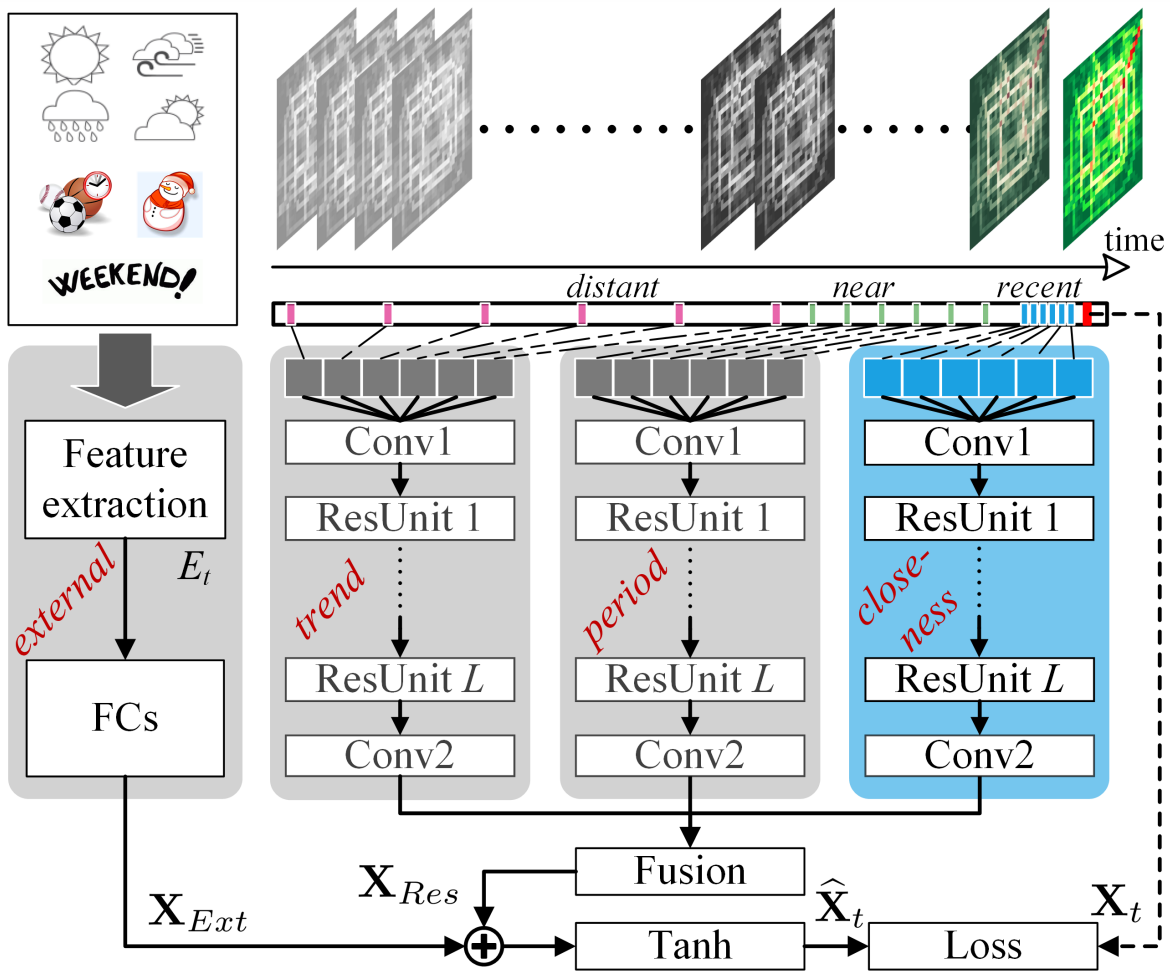
\includegraphics[width=0.8\textwidth,height=10cm,keepaspectratio=true]{content/images/STResNetArchitecture.png}
    \caption{Architektur von ST-ResNet \cite[Figure 3]{STResNetOriginal}}
    \label{fig:STResNetArchitecture}
\end{figure}

ST-ResNet besteht im Wesentlichen aus vier Teilen, die in \autoref{fig:STResNetArchitecture} eingerahmt sind.
Die drei rechten Teile modellieren den langfristigen Trend (\emph{trend}), mittelfristige Periodizitäten (\emph{period}) und kurzfristige Begebenheiten (\emph{closeness}).
Diese drei Teile haben jeweils die gleiche Struktur.
Die Eingangsdaten werden zunächst einem \acrshort{cnn}-Layer zugeführt.
Dessen Ausgabe durchläuft dann mehrere sogenannte Residual Units.
Diese beinhalten wiederum \acrshort{cnn}-Layer, jedoch wird die Eingabe einer Residual Unit wieder zum Ausgang der \acrshort{cnn}-Layer dazuaddiert.
Dadurch können sehr tiefe Netze gebildet werden, ohne dass diese dem Problem des verschwindenden Gradienten unterliegen.
Der Ausgang der letzten Residual Unit wird schlussendlich nochmals durch einen \acrshort{cnn}-Layer verarbeitet.

Der Unterschied dieser drei rechten Teile liegt in den Eingangsdaten.
Der \emph{trend}-Teil erhält als Eingangsdaten Zeitschritte im Abstand von einer Woche, die über die gesamte Zeitspanne des Datensatzes verteilt sind.
Somit kann die langfristige Entwicklung der Daten erlernt werden, wie auch wöchentliche Periodizitäten.
Der \emph{period}-Teil erhält Zeitschritte im Abstand von einem Tag, die nicht sehr lange zurückliegen.
Damit können tägliche Periodizitäten erlernt werden, wie die bereits erwähnten Stoßzeiten.
Zuletzt erhält der \emph{closeness}-Teil alle verfügbaren Zeitschritte der letzten paar Tage.
Anhand dessen kann die momentane Situation erkannt werden.
Diese Ausgaben dieser drei Teile werden schlussendlich gewichtet zusammengeführt.
Der in \autoref{fig:STResNetArchitecture} ganz links dargestellte Teil verarbeitet externe Daten durch ein vollständig verbundenes Netz.
Signifikante Merkmale, die als Eingabe dienen sollen, müssen hierfür manuell ermittelt werden.
Die Kombination aus dem linken Teil und der zusammengeführten Ausgabe der drei rechten Teile bildet schließlich die Ausgabe von ST-ResNet.

\textbf{ConvLSTM} ist ebenfalls eine weit verbreitete Architektur für räumlich-zeitliche Vorhersagen.
Conv\-LSTM wurde von Shi et al. in \cite{ConvLSTM} vorgestellt.
Bei ConvLSTM handelt es sich um eine Kombination aus \acrshort{cnn} und \acrshort{lstm}.
Durch Faltungsoperationen soll hierbei die räumliche Strukur erhalten bleiben.
Außerdem soll durch die Verwendung einer abgewandelten \acrshort{lstm}-Struktur die zeitlichen Zusammenhänge erfasst werden.
Das ursprüngliche Ziel von ConvLSTM ist nach Shi et al. die Vorhersage einer \emph{Sequenz} von 2D-Daten anhand einer Eingabesequenz.
Dafür orientieren sie sich an der in \cite{SequenceGeneratingLSTM} vorgestellten Architektur.
Diese Architektur besteht aus mehreren hintereinandergeschalteten \acrshort{lstm}-Zellen.
Jedoch wurde sie für die Generierung von 1D-Sequenzen konzipiert und verwendet daher Matrixmultiplikationen mit Gewichtungsmatrizen.
Diese werden von Shi et al. durch Faltungsoperationen ersetzt, wodurch zweidimensionale Strukturen erlernt werden können.
Diese Architektur wird in \autoref{fig:ConvLSTMStructure} verdeutlicht.

\begin{figure}[h]
    \centering
    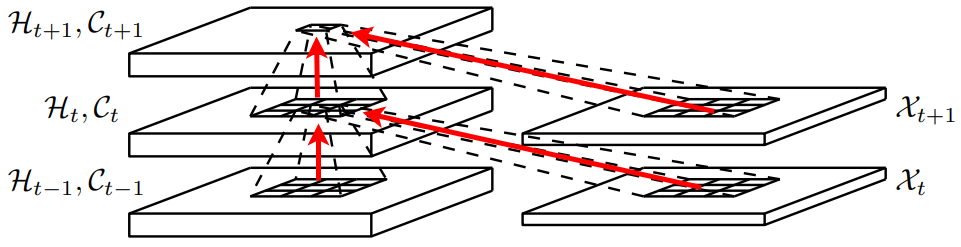
\includegraphics[width=0.8\textwidth,height=10cm,keepaspectratio=true]{content/images/ConvLSTMStructure.png}
    \caption{Innere Struktur von ConvLSTM aus \cite{ConvLSTM} mit hinzugefügten Pfeilen zur Verdeutlichung des Informationsflusses}
    \label{fig:ConvLSTMStructure}
\end{figure}

Wie man in der Abbildung erkennen kann, hängt jedes Pixel der Ausgabe von einem Bereich der Eingabe und einem Bereich des inneren Zustands ab.
Dadurch, dass die Tore aus der \acrshort{lstm}-Architektur übernommen wurden, werden von ConvLSTM auch die räumlich-zeitlichen Zusammenhänge nach ihrer Relevanz gefiltert.
Der große Vorteil von ConvLSTM besteht darin, dass es bereits eine fertige Implementierung als Teil von TensorFlow gibt.


% Warum für eins entschieden?
% Verwandte Anwendungsfälle:
%   - Niederschlagsvorhersage als weiter entfernt
%   - Verbrechensvorhersage als sehr ähnlichen Anwendungsfall
